\documentclass{article}
\usepackage[utf8]{inputenc}
\usepackage{graphicx}
\usepackage{float}
\usepackage{datetime}
\usepackage{alltt, fancyvrb, url}
\usepackage{hyperref}
\usepackage{csquotes}
\usepackage{tikz} % grafici
\usepackage{adjustbox}
\usepackage{mdframed}

\usepackage{ifthen} %esecuzioni condizionali
\usepackage{algorithmicx} %algoritmi
\usepackage{algpseudocode} %costrutti pseudocodice
\usepackage{listings} %porzioni di codice 
\usepackage{xfp} %per moltiplicazioni

%DECOMMENTA SE VUOI FARE CITAZIONI
%\usepackage[style=verbose-ibid,backend=biber]{biblatex} %per la bibliografia con \cite, \footcite, ecc.
\usepackage[italian]{babel}
\usepackage{xurl} %per linkare url con \url{}
\usepackage{amsmath} % pacchetto per le equazioni matematiche
\usepackage{amsthm}
\theoremstyle{definition}
% Definizione dell'ambiente per le definizioni
\newtheorem{definizione}{Definizione}

\usepackage{amssymb}
\usepackage{biblatex}
\usepackage[italian]{cleveref} % pacchetto per i riferimenti incrociati

\addbibresource{bibliography.bib}

\title{Dimostrazione a conoscenza zero \\
        \large
        Corso di Crittografia A.A. 2022/23}
\author{Mattia Panni}
\date{\today}

\begin{document}

\maketitle
\clearpage
\tableofcontents
\clearpage

\section{Introduzione}
Le dimostrazioni a conoscenza zero (\emph{zero-knowledge proofs}) rappresentano un potente strumento crittografico e concettuale utilizzato per dimostrare la conoscenza di una determinata informazione senza rivelarla effettivamente. In altre parole, consentono a una parte, chiamata ``\emph{prover}'' (che da qui in avanti definiremo come $P$), di dimostrare di possedere una \emph{conoscenza} specifica (tipicamente chiamata \emph{witness} o \emph{testimone} in letteratura) a un'altra parte, chiamata ``\emph{verifier}'' ($V$), senza rivelare i dettagli di tale conoscenza. Le zero-knowledge proofs sono ampiamente utilizzate in diversi campi, come la sicurezza informatica, la crittografia e la privacy. Queste dimostrazioni offrono la possibilità di verificare l'autenticità o la veridicità di una dichiarazione senza rivelare informazioni sensibili o segrete. Le zero-knowledge proofs sono state oggetto di intensa ricerca e sviluppo, portando a protocolli e algoritmi sempre più sofisticati che garantiscono la sicurezza e la privacy delle transazioni e delle comunicazioni. Oltre a questo, ricoprono un ruolo fondamentale nell'ambito dell'informatica teorica, specialmente nel campo della \emph{Teoria della Complessità Computazionale}. Ad esempio dimostrando l'equivalenza fra classi di problemi differenti quali \texttt{$\mathcal{IP}$} e \texttt{$\mathcal{PSPACE}$}. Nelle prossime sezioni verranno trattate queste dimostrazioni-, nonché il loro legame con la classe di problemi \texttt{$\mathcal{IP}$} e la loro potenza computazionale paragonabile a quella di macchine di Turing con una quantità di memoria polinomiale.

\subsection{Storia}
Le Zero-Knowledge Proofs (ZKP), ovvero le dimostrazioni a conoscenza zero, sono state sviluppate come risultato di un'intensa ricerca nel campo della crittografia e dell'informatica teorica. L'idea di dimostrazioni a conoscenza zero ha cominciato a prendere forma negli anni '80 grazie ai lavori di pionieri come Shafi Goldwasser, Silvio Micali e Charles Rackoff nell'articolo ``\emph{The Knowledge Complexity of Interactive Proof-System}''\cite{micali} in cui venivano trattate uno specifico tipo di dimostrazioni, dette \emph{interattive}. 
Da quella scoperta fondamentale, la comunità scientifica ha dedicato considerevole impegno allo sviluppo e all'avanzamento delle Zero-Knowledge Proofs (ZKP). Negli ultimi decenni, sono emerse varie tecniche e protocolli più sofisticati per implementare e utilizzare le ZKP in diversi contesti. Tra queste, zk-SNARK (Zero-Knowledge Succinct Non-Interactive Argument of Knowledge), che ha guadagnato notevole attenzione e popolarità. Lo zk-SNARK è una forma di ZKP che consente di dimostrare la conoscenza di una soluzione senza richiedere interazioni ripetute tra $P$ e $V$, rendendo le dimostrazioni più efficienti e consentendo una vasta gamma di applicazioni pratiche.

\subsection{Fondamenti teorici}
Di seguito vengono riportati dei risultati matematici che consentono di spiegare adeguatamente le ZKP.

\subsubsection{Alfabeti e linguaggi}\label{alfabetilinguaggi}
Il primo elemento chiave nella comprensione delle dimostrazioni a conoscenza zero è quello di \emph{alfabeti} e \emph{linguaggi}. 
Formalmente 
\begin{itemize}
    \item Un \emph{alfabeto}, denotato con la lettera greca $\Sigma$, è un insieme finito e non vuoto, i cui elementi vengono tipicamente chiamati \emph{caratteri}. Un esempio di alfabeto può essere quello binario, cioè 
    \begin{equation*}
        \Sigma = \left\{ 0, 1 \right\}
    \end{equation*} 
    \item Una \emph{stringa} $X$ è una qualsiasi sequenza finita di caratteri, tutti appartenenti allo stesso alfabeto. Il numero di caratteri che la compongono verrà indicato con $| X |$. Denoteremo con $\epsilon$ una stringa vuota.
    \item L'insieme di tutte le possibili stringhe appartenenti allo stesso alfabeto costituiscono un \emph{linguaggio}. Se $\Sigma$ è un alfabeto, allora denoteremo con $\Sigma^*$ l'insieme di tutte le stringhe generabili dagli elementi contenuti in $\Sigma$. Ad esempio
    \begin{equation*}
        \left\{ 0, 1 \right\}^* = \left\{\epsilon, 0, 1, 00, 10, 11, 000, \dots \right\}
    \end{equation*}
\end{itemize}
Per gli scopi di questo elaborato e senza perdere di generalità, un linguaggio è un insieme di oggetti o di istanze che soddisfano una certa proprietà o condizione specifica. Ad esempio, potremmo avere un linguaggio di istanze booleane, in cui le istanze sono semplici espressioni booleane e il linguaggio comprende tutte le istanze che valutano a ``vero''. Oppure potremmo avere un linguaggio di grafi ``hamiltoniani'', in cui le istanze sono grafi e il linguaggio include tutti i grafi che contengono un percorso hamiltoniano\footnote{Un grafo presenta un cammino hamiltoniano se esiste un percorso che tocca tutti i vertici del grafo una ed una sola volta. Formalmente corrisponde a una permutazione $(p_0, p_1, \cdots, p_{n-1})$ di tutti i vertici del grafo tale per cui esista un arco per ogni coppia di nodi adiacenti che li colleghi, cioè $(p_i, p_{i+1}) \in E$ con $0 \leq i \leq n-2$.}. La scelta del linguaggio dipende dal problema specifico che si intende dimostrare o verificare.


\subsubsection{Macchine di Turing interattive}\label{turing}
I \emph{sistemi a dimostrazione interattiva}, che vedremo in seguito, hanno come base teorica degli specifici \emph{automi a stati finiti}, chiamati \emph{macchine di Turing interattive}.
Come indica la figura \ref{fig:fsm}, un automa a stati finiti (anche detto Finite State Machine, FSM) è un modello matematico che rappresenta un sistema che si trova in uno stato specifico e può effettuare una transizione da uno stato all'altro in risposta a degli input. Questi FSM sono tipicamente utilizzati per descrivere il comportamento di sistemi complessi che transitano da uno stato ad un altro a causa di specifici eventi. Dal nome si comprende come il numero di stati in cui può trovarsi deve essere finito.

\begin{figure}[H]
    \centering
        \begin{tikzpicture}
          % Definizione dei nodi
          \node[circle, draw, double, inner sep=3pt] (S1) at (0,0) {S1};
          \node[circle, draw] (S2) at (2.5,0) {S2};
        
          % Definizione degli archi
          \draw[->] (-1,0) -- (S1); % Arco entrante in S1
          \draw[->] (S1) edge[bend left] node[midway, above] {0} (S2); % Arco da S1 a S2 con peso 0
          \draw[->] (S2) edge[bend left] node[midway, below] {0} (S1); % Arco da S2 a S1 con peso 0
          \draw[->] (S1) edge[loop left, out=120, in=60, looseness=5] node[midway, above] {1} (S1); % Arco da S1 a S1 con peso 1 (in alto)
          \draw[->] (S2) edge[loop right] node[midway, right] {1} (S2); % Arco da S2 a S2 con peso 1
        \end{tikzpicture}
    \caption{Esempio di automa a stati finiti.}
    \label{fig:fsm}
\end{figure}

La \emph{Macchina di Turing} (ideata dall'omonimo nel 1936) consiste in un'astrazione matematica rappresentate un computer ideale con una memoria infinita e un'unità di controllo programmabile. La macchina di Turing è composta da una testina che può leggere e scrivere su un nastro di memoria suddiviso in celle, una regola di transizione che specifica come la macchina si comporta in base allo stato corrente e al simbolo letto, e uno stato interno che può cambiare in base alle regole di transizione. In questo senso la macchina di Turing rappresenta un'estensione delle FSM in quanto può potenzialmente supportare infiniti stati e eseguire azioni quali lo spostamento della testina programmandone un'unità di controllo.

Un'ulteriore estensione delle macchine di Turing è rappresentata dalle \emph{Macchine di Turing interattive} (ITM) in cui la casualità gioca un ruolo estremamente importante.
Infatti esse dispongono di un nastro specifico detto \emph{random} che rappresenta una fonte di casualità sotto forma di infinita sequenza di bit random. Ad ogni iterazione la macchina sposta la testina da destra a sinistra e legge il bit successivo. Assumendo che la sequenza sia effettivamente casuale\footnote{In realtà essendo pseudocasuale, cioè simulata da un algoritmo deterministico, a seconda di come si sceglie il seme, la sequenza risulterà riproducibile e dunque non random.}, possiamo assumere che la probabilità di estrarre un bit rispetto ad un altro a seguito di una lettura sarà pari a quella che ho nell'ottenere testa a seguito del lancio di una moneta non truccata e cioè
\begin{equation*}
    Pr\left(\text{bit} = 1\right) = Pr\left(\text{Testa}\right) = \frac{1}{2}
\end{equation*}
Esse poi presentano un nastro di input da cui leggono informazioni spostando la testina, un nastro di lavoro su cui possono fare le loro computazioni e uno di scrittura.

\paragraph{Coppia di macchine interattive}
Al fine di spiegare formalmente le dimostrazioni interattive, è necessario spiegare il funzionamento di coppie di \emph{macchine di Turing interattive}, cioè di come due ITM interagiscono fra loro. Definiamo due macchine di Turing interattive $A$ e $B$, esse costituiscono un coppia $(A, B)$ se
\begin{enumerate}
    \item si impone che $A$ e $B$ condividano lo stesso nastro di input 
    \item il nastro di sola scrittura di $B$ sia il nastro di sola lettura di $A$ e viceversa
\end{enumerate}
Va sottolineato che la coppia è ordinata, cioè le due ITM operano a turni alterni. Durante il proprio turno, ad esempio $A$, legge dal nastro di lettura, effettua delle operazioni sul proprio nastro di lavoro e infine comunica a $B$ quanto fatto scrivendo sul proprio nastro di scrittura (che per la (2) corrisponde al nastro di lettura di $B$).
Ad ogni turno una macchina può interrompere l'interazione della coppia.

Questa iterazione può essere riassunta nella figura seguente, riadattata da \cite[p. 292]{micali}
\begin{figure}[H]
    \centering
    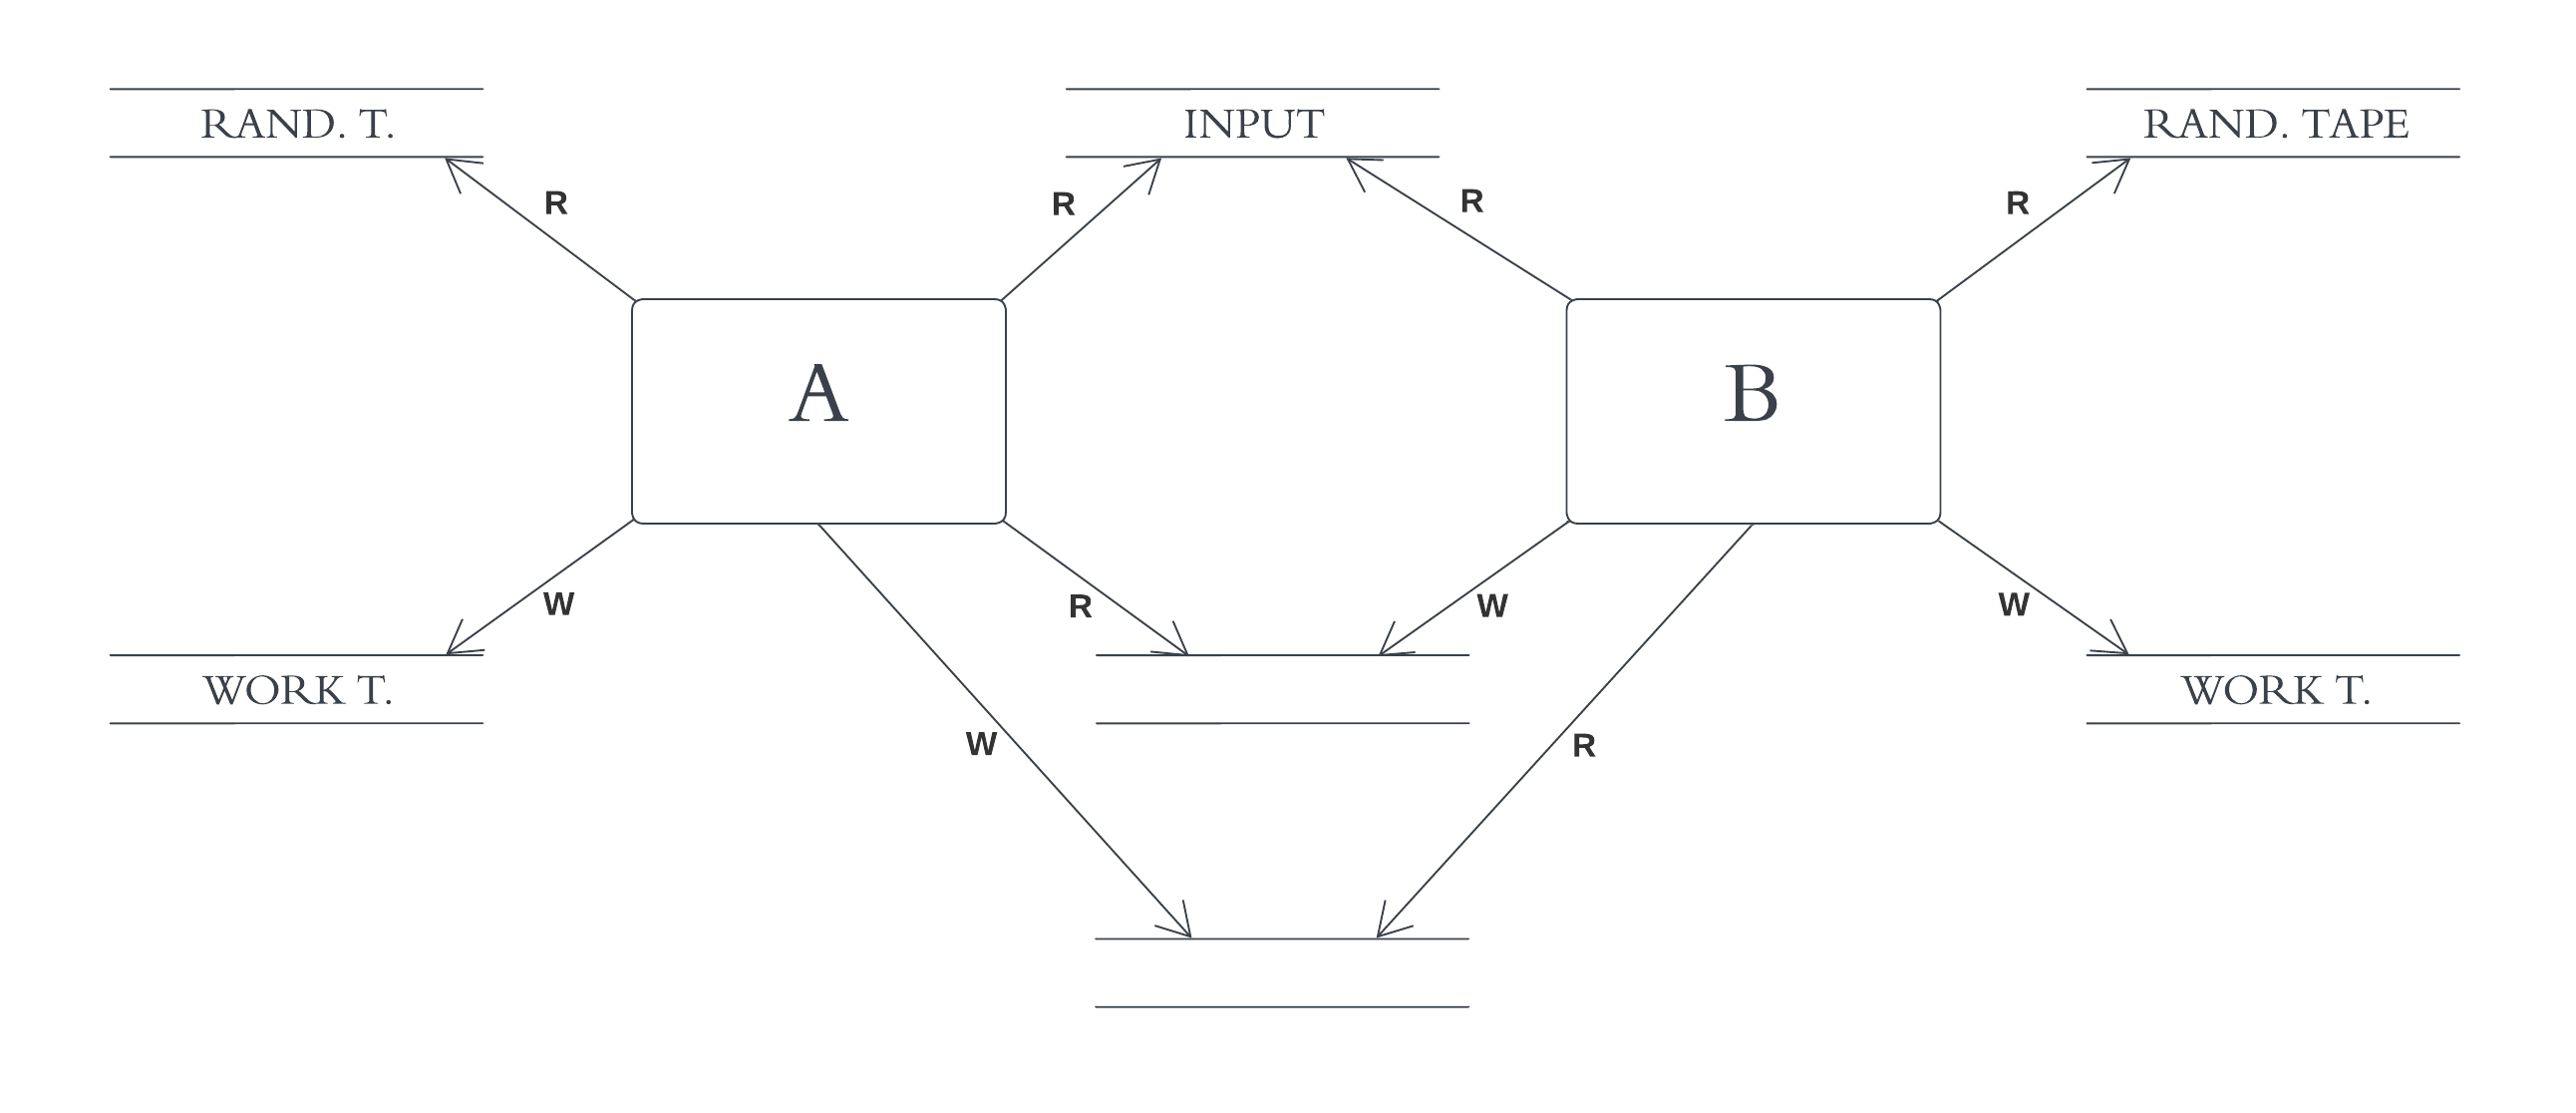
\includegraphics[width=\textwidth]{imgs/ITM.png}
    \caption{Interactive Turing Machine.}
    \label{fig:itm}
\end{figure}

Per quanto detto un'interazione è rappresentata da al più $n$ coppie di scambi di messaggi $(a_i, b_i)$ con $i = 1, \dots, n$, dove $a_i$ corrisponde all'$i-$esimo messaggio di $A$ e similmente $b_i$.
Dunque il testo risultante da una computazione sull'input $x$ in cui parte $B$ per primo, avrà la seguente forma
\begin{equation*}
    \left\{ b_1, a_1, b_2, a_2, \cdots, b_n, a_n \right\}
\end{equation*}
in cui $a_n$ vuota se $B$ ha terminato la computazione della coppia al suo $n-$esimo turno.
La ``randomness'' entra in gioco nella decisione di che tipo di computazione eseguire prima di inserire il messaggio $i-$esimo nel nastro. In questo senso, l'insieme di tutti i testi generati dalle computazioni di $A$ e $B$ a partire da un dato input $x$ costituisce uno spazio di probabilità che denoteremo come $(A, B)[x]$.

\subsubsection{Teoria della complessità computazionale}\label{complessita}
Lo scopo di questa disciplina nell'ambito dell'informatica teorica è quello di esaminare e classificare i problemi computazionali in base alle risorse richieste per risolverli (che sia in termini di spazio o di tempo). Questa è una sfida complessa perché potremmo intuitivamente pensare che il numero di risorse utilizzate dipenda dall'algoritmo scelto. Potrebbe essere possibile risolvere un problema in modo efficiente, ma se non conosciamo un algoritmo che lo permetta, potremmo essere costretti a impiegare molte risorse. In realtà si è scoperto che ogni problema possiede una sua \emph{complessità computazionale} intrinseca (cioè che rimane tale anche scegliendo l'algoritmo migliore). 
\paragraph{Tipologie di problemi}
Esistono diverse tipologie di problemi, ciascuna con le sue caratteristiche distintive:
\begin{itemize}
    \item \emph{Problemi decisionali}. Sono problemi i cui risultati possibili sono solo  ``si'' o ``no''. Possiamo rappresentare questi problemi come linguaggi formali (si veda paragrafo \ref{alfabetilinguaggi}) 
    in cui le istanze\footnote{L'istanza di un problema è un esempio specifico del problema, che può essere visto astrattamente come l'insieme di tutte le sue istanze. In altre parole è un input concreto del problema.} che producono l'output ``si'' appartengono al linguaggio. Ad esempio se $L = \left\{ \text{numeri pari} \right\}$, dato un numero $x$ si ha che
    \begin{align*}
    \begin{cases}
    x \in L \Leftrightarrow x \text{ è divisibile per }2\\
    x \notin L \text{ altrimenti}
    \end{cases}
    \end{align*}
    \item \emph{Problemi di funzione}. In essi, l'output fornito a seguito dell'applicazione della soluzione (che possiamo associare a una funzione $f$) verrà fornito un output ben più complesso del semplice ``si'', ``no'' dei decisionali. Un noto esempio in letteratura è \emph{problema del commesso viaggiatore}\footnote{Dato un elenco di città con le distanze fra ogni coppia di queste, determinare qual'è il percorso più breve che da una città di partenza le percorra tutte una volta e si concluda nella città di partenza.}.
\end{itemize} 
Esistono altre tipologie di problemi che non sono rilevanti per questa trattazione.

\paragraph{Classi di complessità}
Una \emph{classe di complessità} è un insieme di problemi di complessità correlata. Ai nostri scopi le classi verranno caratterizzate dai seguenti fattori
\begin{itemize}
    \item Il tipo di problema computazionale. Tipicamente i più comuni sono quelli decisionali ma alcune classi sono definite per altre tipologie.
    \item Il modello di computazione. Il più comune è la macchina di Turing (Si veda paragrafo \ref{turing}).
    \item La risorsa che viene limitata e il suo limite.
\end{itemize}
Detto questo, vengono di seguito riportate una serie di classi con le rispettive caratteristiche
\begin{itemize}
    \item \texttt{$\mathcal{P}$}: La classe dei problemi che possono essere risolti in tempo polinomiale da una macchina di Turing deterministica. Sono i problemi considerati ``facili'' da risolvere in pratica. 
    \item \texttt{$\mathcal{NP}$}: La classe dei problemi per i quali una soluzione proposta può essere verificata in tempo polinomiale da una macchina di Turing deterministica. Non si conosce un algoritmo efficiente per la loro soluzione, ma se si ottiene una soluzione, è possibile verificarla rapidamente.
    \item \texttt{$\mathcal{NP}$-completo}: Una classe di problemi all'interno di \texttt{$\mathcal{NP}$} che sono considerati tra i più difficili nella teoria della complessità. Un problema \texttt{$\mathcal{NP}$-completo} può essere ridotto\footnote{Una riduzione è una trasformazione di un problema in un altro, che cattura l'idea intuitiva che un problema sia al massimo altrettanto difficile di un altro. Ad esempio, se un problema X può essere risolto utilizzando un algoritmo per il problema Y, allora X non è più difficile di Y e si dice che X si riduce a Y.} a qualsiasi altro problema \texttt{$\mathcal{NP}$} in tempo polinomiale, il che implica che se uno di essi viene risolto in tempo polinomiale, allora tutti i problemi \texttt{$\mathcal{NP}$} possono essere risolti in tempo polinomiale.
    \item \texttt{$\mathcal{NP}$-hard}: Una classe di problemi che sono almeno altrettanto difficili quanto i problemi \texttt{$\mathcal{NP}$-completi}, ma non necessariamente appartenenti a \texttt{$\mathcal{NP}$}. 
    \item \texttt{$\mathcal{PSPACE}$}: La classe dei problemi che possono essere risolti utilizzando una quantità di spazio di memoria polinomiale su una macchina di Turing deterministica. Include molti problemi di decisione e problemi di ricerca nello spazio degli stati.
\end{itemize}

\subsubsection{Algebra modulare}
Dato un numero intero positivo $n$ definiamo con 
\begin{equation*}
    \mathbb{Z}_n = \{0,1,\dots ,n-1\}
\end{equation*}
l'insieme dei numeri interi non negativi minori di $n$. 
Ad esempio per $n = 6$ avremo $\mathbb{Z}_6 = \{0,1,2,3,4,5\}$.
Definiamo ora $\mathbb{Z}_n^*$ come l'insieme degli elementi di $\mathbb{Z}_n$ \emph{relativamente primi} con $n$ (0 escluso, 1 incluso). Si dice che
\begin{equation*}
    a \text{ è relativamente primo con } b \Leftrightarrow MCD(a, b) = 1
\end{equation*}
cioè non hanno divisori comuni eccetto l'1.
Continuando l'esempio con $n = 6$, $\mathbb{Z}_n^*$ sarebbe composto da tutti quei numeri primi con 6, cioè quei numeri il cui massimo comune divisore con 6 è 1 (ovvero non hanno divisori comuni). Pertanto
$\mathbb{Z}_6^* = \{1,5\}$.
Se invece prendiamo un numero primo come 7, avremo $\mathbb{Z}_7^* = \{1,2,3,4,5,6\}$ poiché chiaramente, essendo primo, il massimo comune divisore fra quel numero e uno più piccolo sarà sicuramente 1 non avendo dei fattori moltiplicativi che lo originano. 
Pertanto $\mathbb{Z}_n^*$ di un numero primo $p$, che ragionevolmente indicheremo con $\mathbb{Z}_p^*$ sarà dato da
\begin{equation*}
    \mathbb{Z}_p^* = \{1, \dots, p-1\}
\end{equation*}

Dopo aver fatto questa premessa introduciamo il concetto di \emph{modulo}. Sia

\begin{equation*}
    a \bmod n
\end{equation*}
il resto della divisione intera fra $a$ e $n$. Cioè immagino di spezzare $a$ in $n$ parti uguali. L'ultima parte, se più piccola di $n$, avanzerà e costituirà proprio questa quantità.

\paragraph{Proprietà aritmetiche del modulo}
Tutte le operazioni aritmetiche di somma, prodotto, differenza e divisione, possono essere fatte distribuendo il modulo sui termini che compaiono. In altre parole, vale la proprietà distributiva con il modulo.
Ad esempio si ha
\begin{align*}
    &(a + b) \bmod n = ((a \bmod n) + (b \bmod n)) \bmod n \\ 
    &(a - b) \bmod n = ((a \bmod n) - (b \bmod n)) \bmod n \\
    &(a \times b) \bmod n = ((a \bmod n) \times (b \bmod n)) \bmod n \\
    &a^{r \times s} \bmod n = ((a^r \bmod n)^s) \bmod n, \quad \text{ con } r,s \text{ interi positivi} 
\end{align*}
Queste proprietà servono poiché a volte può essere utile (ad esempio per esigienze computazionali) distribuire il modulo fra fattori di dimensione più piccola.

\paragraph{Congruenza}
Si parla di \emph{congruenza} fra $a$ e $b$ mod $n$, esprimendola come
\begin{equation*}
    a \equiv b \bmod n \Leftrightarrow a \bmod n = b \bmod n
\end{equation*}
Cioè $a$ è congruente con $b$ se e solo se, qualora li dividessi per lo stesso numero $n$, generino lo stesso resto (pur non essendo necessariamente uguali). In questo caso si dice che appartengono nella stessa \emph{classe di equivalenza}.
Per fare un esempio risulta $5 \equiv 11$ mod $3$, poiché sia 5 che 11, se divisi per 3 danno come resto 2.
Alternativamente si può scrivere 
\begin{equation*}
    a \equiv b \bmod n \Leftrightarrow a = b + kn
\end{equation*}
Cioè $a$ è dato dalla somma di $b$ e un multiplo di $n$. Infatti se scrivo $7 \equiv 1$ mod $3$, allora sto dicendo che $7 = 1 + k3$, con $k = 2$.

Introduciamo ora dei concetti che ci saranno utili in seguito.
\begin{itemize}
    \item \emph{Inverso moltiplicativo}. Dato un numero $a$ e un modulo $n$, l'inverso moltiplicativo di $a$ è un numero $b$ tale che $ab \equiv 1 \bmod n$. In altre parole, $b$ è un numero che moltiplicato per $a$ produce un multiplo di $n+1$. Ad esempio, l'inverso moltiplicativo di 3 modulo 5 è 2, poiché $3 \times 2 \equiv 1 \bmod 5$.
    \item \emph{Radice quadrata modulo $n$}. Dato un numero $a$ e un modulo $n$, la radice quadrata modulo $n$ di $a$ è un numero $b$ tale che $b^2 \equiv a \bmod n$. Ad esempio, la radice quadrata modulo 5 di 4 è 2, poiché $2^2 \equiv 4 \bmod 5$.
    \item \emph{Residuo quadratico}. Dato un numero $a$ e un modulo $n$, $a$ è un residuo quadratico modulo $n$ se esiste un numero $b$ tale che $b^2 \equiv a \bmod n$. Ad esempio, 4 è un residuo quadratico modulo 5, poiché $2^2 \equiv 4 \bmod 5$.
\end{itemize}



\subsection{Sistemi a dimostrazione interattiva}
I primi ad essere presentati vengono detti \emph{sistemi a dimostrazione interattiva} il cui nome suggerisce la presenza di interazione tra un prover e un verifier. Questa modalità rende più semplice comunicare una qualche informazione. Citando Micali ``\emph{Ci occupiamo di quelle prove che possono essere ``spiegate in classe''. In modo informale, in una classe, il docente può sfruttare appieno la possibilità di interagire con i ``destinatari'' della prova. Essi possono porre domande nei punti cruciali dell'argomentazione e ricevere risposte. Questo rende la vita molto più facile.}'' \cite{micali}.


Formalmente disponiamo di una coppia di macchine di Turing interattive $(P, V)$, ciascuna con una specifica potenza computazionale. In particolare 
\begin{itemize}
    \item Il \emph{prover} $P$, responsabile di dimostrare di possedere una determinata informazione (o \emph{witness}), ha una \emph{potenza computazionale infinita}, superando la capacità di una normale macchina di Turing.
    \item Il \emph{verifier} $V$, il cui compito è essere convinto dal prover che quest'ultimo possiede effettivamente la witness, ha una \emph{potenza computazionale polinomiale}, ossia è implementato da un algoritmo polinomiale.
\end{itemize}
Definiamo ora un linguaggio $L \subseteq \left\{ 0,1 \right\}^*$ delle stringhe binarie di lunghezza arbitraria, tale che
\begin{enumerate}
    \item Esiste un prover $P$ tale che, se $x \in L$, allora la probabilità che l'interazione fra $P$ e $V$ porti il verifier ad accettare è almeno pari a $1 - \frac{1}{n^k}$, in altre parole
    \begin{equation*}
        \exists P : x \in L \Rightarrow Pr\left(P \leftrightarrow V\text{ accetta } x\right) \geq 1 - \frac{1}{n^k} 
    \end{equation*}
    per ogni $k$ (dove $k$ corrisponde all'iterazione corrente dell'algoritmo) e $n$ (dove $n = |x|$, cioè corrisponde alla lunghezza dell'input), sufficientemente grande.
    \item Per ogni prover $\Tilde{P}$ tale che, se $x \notin L$, allora la probabilità che l'interazione fra $\Tilde{P}$ e $V$ porti $V$ ad accettare con probabilità al massimo $\frac{1}{n^k}$, cioè
    \begin{equation*}
        \exists \Tilde{P} : x \notin L \Rightarrow Pr\left(P \leftrightarrow V\text{ accetta } x\right) \leq \frac{1}{n^k} 
    \end{equation*}
    per ogni iterazione $k$ e per $n$ sufficientemente grande.
\end{enumerate}
In quanto detto, le probabilità sono calcolate sul lancio della moneta di $V$ (cioè all'estrazione di $k$ bit casuali dal nastro random).

Quando detto può essere riassunto in due proprietà fondamentali che ogni sistema a dimostrazione interattiva deve possedere
\begin{itemize}
    \item \emph{Completezza} (``completeness''). Il verifier deve sempre essere aperto ad accettare una dimostrazione veritiera. In altre parole deve esistere una strategia del prover che, a seguito dell'interazione fra $P$ e $V$ su un input comune $x \in L$, porti il verifier ad accettarla con probabilità schiacciante.
    In altre parole, è possibile dimostrare un teorema vero in modo che le prove siano facilmente verificabili ($V$ è in tempo polinomiale).
    \item \emph{Correttezza} (``soundness''). Se $x \notin L$, non esiste alcuna strategia per convincere $V$ del contrario, che abbia successo con probabilità non trascurabile. In altre parole, non si può dimostrare un teorema falso.
\end{itemize}
\subsubsection{Dimostrazioni interattive in \texorpdfstring{\texttt{$\mathcal{NP}$}}{NP}}
 Quando si considera la classe di problemi $\mathcal{NP}$ (si veda la sezione \ref{complessita}), esistono sistemi di dimostrazione interattivi specifici, chiamati in letteratura "sistemi di dimostrazione interattivi $\mathcal{NP}$'' (\emph{\texttt{$\mathcal{NP}$}-proof systems}). A differenza di quelli che vedremo in seguito, questi sistemi a potenza limitata non si affidano alla ``randomness'' messa a disposizione al verifier (attraverso il lancio della moneta). Inoltre limitano l'interazione fra $P$ e $V$ ad un solo scambio di informazioni. 
Questo tipo di dimostrazioni vengono chiamate \texttt{$\mathcal{NP}$} dal momento che, come mostrato nel paragrafo \ref{complessita}, questa classe di complessità comprende tutti quei problemi una cui soluzione non è determinabile in tempo polinomiale ma la cui dimostrazione di correttezza di una data soluzione (inviata nel caso di questi sistemi da $P$ a $V$), è ottenibile in tempo polinomiale.
I requisti di completezza e correttezza citati in precedenza, in questo caso sono rispettati in maniera triviale dal momento che non vi è aleatorietà, dunque
\begin{align*}
    &\exists P : x \in L \Rightarrow Pr\left(P \leftrightarrow V\text{ accetta } x\right) = 1 \\
    &\forall \Tilde{P} : x \notin L \Rightarrow Pr\left(P \leftrightarrow V \text{ accetta } x\right) = 0
\end{align*}

\paragraph{Esempio 1}
Definiamo un linguaggio $L = \text{SAT}$, corrispondente all'insieme delle espressioni booleane soddisfacibili. SAT (\emph{Satisfability}) è un problema decisionale molto noto in letteratura appartenente alla classe \texttt{$\mathcal{NP}$}. Questo significa che è computazionalmente complicato determinare una soluzione (che nel caso specifico equivale ad un assegnamento delle variabili booleane in gioco che renda vera la formula) al problema, ma è molto facile verificare che un determinato assegnamento soddisfi l'intera formula.
Nel concreto la coppia $(P, V)$ opera su un'espressione in input $x$. L'interazione consiste in una singola mossa con cui $P$ manda a $V$ una stringa $y$ che corrisponde ad un assegnamento alle variabili della formula. Nel contesto dei problemi \texttt{$\mathcal{NP}$} questa stringa è anche detta \emph{certificato}.
Se l'espressione $x$ è soddisfacibile (cioè $x \in L$) il prover può dimostrarlo inviando al verifier un valido assegnamento. Viceversa se l'espressione non è soddisfacibile ($x \notin L$) non esiste alcun assegnamento $y$ tale che induca $V$ ad accettare.
Considerando una forma particolare di SAT chiamata \emph{3-SAT}, si assume in input una formula 3-CNF che consiste in clausole contenenti solo operazioni di OR, unite tra loro mediante l'operatore di AND. Ogni clausola è composta al massimo da 3 letterali, come ad esempio la seguente formula:
\begin{equation*}
(x_1 \lor \neg x_2 \lor x_3) \land (\neg x_1 \lor x_2 \lor \neg x_3)
\end{equation*}
una possibile stringa $y$ può essere la seguente 
\begin{equation*}
    x_1 = \text{\texttt{true}} \quad x_2 = \text{\texttt{true}} \quad x_3 = \text{\texttt{false}}
\end{equation*}
Un possibile protocollo potrebbe essere schematizzato come segue
\begin{table}[H]
\centering
\begin{tabular}{ccc}
                       & $x$               &              \\
Prover $P$             &                   & Verifier $V$ \\ \hline
$y = \left\{ \text{\texttt{true}}, \text{\texttt{true}}, \text{\texttt{true}} \right\}$ &                   &              \\
                       & $\overset{y} \longrightarrow$ &              \\
                       &                   & check $x(y)$
\end{tabular}
\caption{Esempio di protocollo dimostrazione interattiva SAT.}
\label{tab:protocolnp}
\end{table}
In esso non vi è traccia di randomness o multipli scambi.

\subsubsection{Dimostrazioni interattive in \texorpdfstring{\texttt{$\mathcal{IP}$}}{IP}}


Il lavoro di Micali e dei suoi colleghi ha introdotto una nuova classe chiamata \texttt{$\mathcal{IP}$} (\emph{Interactive Polynomial-time}), che comprende i linguaggi che possono essere risolti\footnote{Cioè per cui esiste una prova di appartenenza per una data stringa $x$.} tramite sistemi a dimostrazione interattiva.
La potenza delle macchine di Turing interattive è pienamente sfruttata in questa classe di problemi. Infatti i sistemi in \texttt{$\mathcal{IP}$} fanno uso della ``randomness'' messa a disposizione alle ITMs (Interactive Turing Machines).
In questi sistemi, sebbene i lower e upper bound per completezza e correttezza possano variare, vengono tipicamente impostati su $\frac{2}{3}$ e $\frac{1}{3}$ rispettivamente. In altre parole 
\begin{align*}
    &\exists P : x \in L \Rightarrow Pr\left(P \leftrightarrow V\text{ accetta } x\right) \geq \frac{2}{3} \\
    &\forall \Tilde{P} : x \notin L \Rightarrow Pr\left(P \leftrightarrow V \text{ accetta } x\right) \leq \frac{1}{3}
\end{align*}

Un risultato significativo è che è stato provato che la classe \texttt{$\mathcal{IP}$} è equivalente a \texttt{$\mathcal{PSPACE}$}, la quale include i problemi risolvibili utilizzando una quantità di memoria polinomiale in base alla dimensione dell'input. Questo risultato conferma ulteriormente come l'interazione e l'uso della "randomness" espandano il potere espressivo di questo linguaggio oltre la classe NP, come se il caso fosse una \emph{fonte aggiuntiva di informazione}.
 Inoltre, ciò implica che i problemi risolvibili mediante dimostrazioni interattive possono essere risolti da una macchina di Turing deterministica con una quantità di memoria polinomiale.



\paragraph{Dimostrazione \texorpdfstring{\texttt{$\mathcal{IP}$}}{IP} \texorpdfstring{$=$}{uguale} \texorpdfstring{\texttt{$\mathcal{PSPACE}$}}{PSPACE}}
Per dimostrare che due classi di complessità, nel nostro caso \texttt{$\mathcal{IP}$} e \texttt{$\mathcal{PSPACE}$}, si equivalgono occorre dimostrare la doppia implicazione 
\texttt{$\mathcal{IP}$} $\subseteq$ \texttt{$\mathcal{PSPACE}$} e \texttt{$\mathcal{PSPACE}$} $\subseteq$ \texttt{$\mathcal{IP}$}. Questo perché se si dimostra che ciascuna classe è contenuta nell'altra, necessariamente le due devono equivalersi. Pertanto abbiamo

\begin{proof}
    \texttt{$\mathcal{IP}$} $\subseteq$ \texttt{$\mathcal{PSPACE}$}. In un protocollo di dimostrazione interattiva, il verifier interagisce con un prover per verificare una data istanza del problema. Per ipotesi abbiamo assunto che $V$ sia una macchina di Turing avente capacità computazionale polinomiale e poiché \texttt{$\mathcal{PSPACE}$} è la classe dei problemi risolvibili da una macchina di Turing deterministica con una memoria polinomiale, possiamo concludere che \texttt{$\mathcal{IP}$} $\subseteq$ \texttt{$\mathcal{PSPACE}$}.

    Formalmente sappiamo che per dimostrare che un determinato input $x$ appartenga a un linguaggio $L \in$ \texttt{$\mathcal{IP}$} (nel contesto delle dimostrazioni interattive, l'obiettivo di $P$ è proprio convincere $V$ che $x \in L$), sarà sufficiente determinare la massima probabilità $z$ con cui una strategia di $P$ riesca a convincere $V$. Formalmente indichiamo questa quantità come
    \begin{equation*}
        z = \underset{P}{\text{max }} Pr\left(V \leftrightarrow P \text{ accetta } x\right)
    \end{equation*}
    dove $V \leftrightarrow P$ indica un'interazione fra prover e verifier.
    Infatti per definizione, se la probabilità di accettazione della prova è $z \geq \frac{2}{3}$ allora siamo certi che $x \in L$, viceversa se $z\leq \frac{1}{3}$, allora sappiamo che $w \notin L$. A questo punto non resta che dimostrare che è possibile calcolare $z$ in 
    \texttt{$\mathcal{PSPACE}$}, ovvero con una macchina di Turing deterministica a memoria discreta.

    Per fare questo immaginiamo di costruire un albero $k-$ario come quello in figura \ref{fig:albero} in cui, ad ogni nodo del livello $i-$esimo corrisponde una sequenza di $i$ messaggi scambiati fra $P$ e $V$ fino a quel momento.
    L'albero potrà avere profondità polinomiale dal momento che, per definizione, gli scambi devono essere in numero polinomiale. Supponiamo di star lavorando con il linguaggio $\left\{0, 1\right\}^n$ di tutte le stringhe binarie di lunghezza $n$. In tal caso potrò, ad ogni iterazione, costruire al massimo $2^n$ stringhe, pertanto ogni nodo avrà al più $2^{n^c}$ figli (per una costante $c$). I valori inseriti all'interno di ciascun nodo corrispondono alla probabilità, arrivati al livello $i-$esimo partendo dalla radice e scendendo lungo i vari nodi predecessori di quello attuale (dunque considerando i primi $i$ messaggi scambiati) che $V$ accetti. In particolare, dunque, si ha che
    \begin{itemize}
        \item I nodi foglia possono assumere valori 0 o 1 a seconda che $V$ rifiuti o accetti la prova.
        \item I nodi interni dove $P$ invia il messaggio $i-$esimo è il \emph{massimo} fra i valori di probabilità dei nodi figli. Questo perché l'obiettivo del prover è massimizzare la probabilità di successo, cioè l'accettazione da parte del verifier. Pertanto, il nodo interno corrispondente a questa scelta sarà assegnato al valore massimo dei nodi figli. In altre parole, il prover sceglierà il cammino che ha la massima probabilità di successo.
        \item I nodi interni dove $V$ invia il suo $i-$esimo messaggio è il valore \emph{medio} dei valori dei nodi figli, dal momento che il verifier cerca di ottenere una decisione più informata sulla validità dell'input. Questo riflette il fatto che il verifier tiene conto delle risposte del prover e cerca di ottenere una valutazione più accurata dell'input basandosi sulle informazioni fornite dal prover.
    \end{itemize}

    \begin{figure}[H]
        \centering
            \begin{tikzpicture}
              \node [circle, draw] (padre) {};
              \node [circle, draw] (figlio1) at (-1.5, -1.5) {};
              \node [circle, draw] (figlio2) at (1.5, -1.5) {};
              \node [circle, draw] (figlio3) at (-3, -3) {};
              \node [circle, draw] (figlio4) at (0, -3) {};
              \node [circle, draw] (figlio5) at (3,-3) {};
              \node [circle, draw] (figlio6) at (-4, -4.5) {0};
              \node [circle, draw] (figlio7) at (-2, -4.5) {1};
              \node [circle, draw] (figlio8) at (-1, -4.5) {1};
              \node [circle, draw] (figlio9) at (1, -4.5) {0};
              \node [circle, draw] (figlio10) at (2, -4.5) {1};
              \node [circle, draw] (figlio11) at (4, -4.5) {0};
        
              \node (altezza0) at (5, 0) {0};
              \node (altezza1) at (5, -1.5) {1};
              \node (altezzai) at (5, -3) {$i$};
              \node (altezzan) at (5, -4.5) {$p(n)$};
              
              \draw (padre) -- (figlio1);
              \draw (padre) -- (figlio2);
              \draw [dashed] (figlio1) -- (figlio3);
              \draw [dashed] (figlio1) -- (figlio4);
              \draw [dashed] (figlio2) -- (figlio5);
              \draw [dashed] (figlio3) -- (figlio6);
              \draw [dashed] (figlio3) -- (figlio7);
              \draw [dashed] (figlio4) -- (figlio8);
              \draw [dashed] (figlio4) -- (figlio9);
              \draw [dashed] (figlio5) -- (figlio10);
              \draw [dashed] (figlio5) -- (figlio11);
        
            \end{tikzpicture}
        \caption{Esempio di albero delle probabilità.}
        \label{fig:albero}
    \end{figure}
    
    Arrivati al nodo radice, il valore di probabilità al suo interno corrisponde alla probabilità massima con cui il prover induce $V$ ad accettare. Poiché l'albero ha dimensione polinomiale, abbiamo concluso la dimostrazione.
\end{proof}

\begin{proof}
    \texttt{$\mathcal{PSPACE}$} $\subseteq$ \texttt{$\mathcal{IP}$}. Questo verso dell'uguaglianza è estremamente complicato da dimostrare formalmente pertanto cercheremo di coglierne solo l'intuizione. La dimostrazione completa è visionabile al \cite{ipeqpspace}. Occorre dimostrare che ogni problema risolvibile in \texttt{$\mathcal{PSPACE}$} può essere ridotto a un protocollo di dimostrazione interattiva. Possiamo fare ciò costruendo un protocollo di dimostrazione interattiva in cui il verificatore simula la macchina di Turing che risolve il problema in \texttt{$\mathcal{PSPACE}$}. Il verificatore può richiedere al dimostratore di fornire passi intermedi della computazione o dimostrare che la soluzione è corretta. In questo modo, possiamo rappresentare ogni problema in \texttt{$\mathcal{PSPACE}$} come un protocollo di dimostrazione interattiva. Nella dimostrazione \cite{ipeqpspace} viene utilizzata l'artimetizzazione di un'espressione booleana della forma
    \begin{equation}\label{eq:tqbf}
        \forall x_1 \exists x_2 \cdots Q_nx_n \phi(x_1, \dots, x_n) 
    \end{equation}
    appartenente al linguaggio \emph{TQBF} (True Quantified Boolean Formulas), estensione del problema SAT citato in precedenza. In esso, infatti, vengono inserite tutte quelle espressioni booleane $\phi$ soddisfacibili ma con ulteriori restrizioni: entrano in gioco anche dei \emph{quantificatori} $Q$, che possono essere di \emph{esistenza} ($\exists$), o di \emph{universalità} ($\forall$). In particolare la \ref{eq:tqbf} può essere tradotta come segue:
    per ogni $x_1$ esiste un $x_2$ tale che $\cdots$ tale che considerato un quantificatore per $x_n$, l'espressione booleana $\phi(x_1, x_2, \dots, x_n)$ è vera.
\end{proof}


\subsubsection{Prove di appartenenza a linguaggio e di conoscenza}
Fino ad ora abbiamo focalizzato la nostra attenzione sulle cosiddette \emph{dimostrazioni di appartenenza a un linguaggio}.
Prendendo come esempio SAT, fornire una dimostrazione per la soddisfacibilità di una formula $x$ è ben diverso dal dichiarare di essere a conoscenza di un assegnamento che renda vera tale formula fornita in input. Nel primo caso parliamo di dimostrazioni di appartenenza a un linguaggio (l'obbiettivo è dimostrare che la stringa $x$ appartiene al linguaggio delle formule booleane soddisfacibili), nel secondo, invece, si tratta di \emph{dimostrazioni di conoscenza}.
Nel contesto appena descritto, l'obbiettivo di $P$ è convincere $V$ di conoscere un assegnamento valido per $x$. In questo caso la soddisfacibilità di $x$ non è in dubbio dal momento che entrambe le parti avviano l'interazione già sapendo che $x$ può essere soddisfatta.
Questa sottile differenza può essere colta meglio pensando che SAT fa parte della famiglia \texttt{$\mathcal{NP}$}. Il fatto che $x$ sia soddisfacibile non implica automaticamente che chiunque possa trovare un assegnamento valido (in un tempo compatibile con le esigenze di utilizzo dell'informazione). Su questo si innestano fra l'altro, \emph{protocolli crittografici di identificazione} come quello di Fiat e Shamir che vedremo nei paragrafi successivi.



\subsubsection{Dimostrazioni a conoscenza zero}\label{zk}
L'idea alla base del lavoro di Micali e dei suoi colleghi fu quella di ``[...] \emph{fornire un nuovo ed efficiente metodo per comunicare una dimostrazione}''\cite[p. 291]{micali}, che riducesse a zero le informazioni superflue comunicate al di fuori dell'evidenza della dimostrazione.


La \emph{privacy} è uno dei fattori chiave che ha portato all'introduzione del concetto di conoscenza zero. Ciò deriva dalla significativa differenza tra dimostrare di possedere una determinata informazione mediante la sua divulgazione come prova e convincere terze parti della propria conoscenza utilizzando una strategia che non sveli direttamente l'informazione stessa. Queste dimostrazioni hanno un impatto notevole nel mondo reale, specialmente nei settori in cui è necessario dimostrare di avere accesso a informazioni sensibili che, per loro natura, non possono essere comunicate.
In altre parole, il prover dimostra di possedere l'informazione senza fornire alcun indizio su di essa. Questo garantisce la confidenzialità della witness e preserva la privacy dell'informazione sensibile che potrebbe essere coinvolta nella dimostrazione.

Come già anticipato, i sistemi a dimostrazione interattiva in \texttt{$\mathcal{IP}$} introducono una componente di probabilità dovuta alla possibilità di leggere un nastro generatore di bit pseudocasuali. Questo comporta che le stringhe prodotte dall'interazione fra le due ITM, seguano una \emph{distribuzione di probabilità}. Questa distribuzione descrive la probabilità relativa che una certa stringa di output si verifichi rispetto alle altre possibili stringhe di output.

Questo aspetto diventa cruciale nel contesto delle Zero-Knowledge Proofs (ZKP), poiché affermare che queste dimostrazioni non trasmettono ulteriore conoscenza oltre alla correttezza della proposizione in questione, significa che, considerando l'interazione tra una coppia di macchine di Turing interattive $(P, V)$ e un estrattore di conoscenza $\hat{V}$\footnote{I \emph{knowledge extractor} sono algoritmi che, dato l'accesso a una conversazione tra prover e verifier, cercano di estrarre la conoscenza posseduta dal prover senza dover effettivamente conoscere l'informazione stessa. L'obiettivo di un knowledge extractor è dimostrare che se un prover può convincere un verifier della veridicità di una proposizione, allora è possibile estrarre o ottenere la prova stessa senza la collaborazione del prover. Questo dimostra che il prover effettivamente possiede la conoscenza richiesta senza rivelarla esplicitamente.}, la distribuzione di probabilità che $\hat{V}$ osserva sui nastri di $P$, risulta essere indistinguibile (come vedremo in seguito, ci sono diverse varianti di questo concetto) dalla distribuzione che può essere calcolata a partire dall'input $x$ in tempo polinomiale. Ciò implica che anche il verificatore (qualora non seguisse il protocollo) non potrebbe estrarre conoscenza aggiuntiva dall'interazione, mantenendo quindi la proprietà di zero knowledge.


\paragraph{Indistinguibilità di variabili casuali}
Supponiamo di lavorare con famiglie di \emph{variabili casuali} $U = \left\{U(x)\right\}$, dove $x$ appartiene al linguaggio $L = \left\{0, 1\right\}^*$.
Ogni $U = \left\{U(x)\right\}$ rappresenta una distribuzione di probabilità delle stringhe generabili dal linguaggio $L$ quando l'input è $x$.
Consideriamo ora due famiglie di variabili casuali $U = \left\{U(x)\right\}$ e $V = \left\{V(x)\right\}$. L'obiettivo è dimostrare che, all'aumentare della dimensione di $x$, queste due distribuzioni diventano \emph{indistinguibili}, il che significa che è possibile scambiare $U(x)$ con $V(x)$ e viceversa.
Per comprendere come ciò sia possibile, immaginiamo di fornire casualmente un campione da una delle due distribuzioni a un ``giudice'' incaricato di determinare a quale famiglia esso appartenga.
In questo contesto, diventa evidente che $U(x)$ può essere sostituito con $V(x)$, al crescere della dimensione di $x$, nel momento in cui il verdetto di qualsiasi giudice non ha più significato, poiché diventa impossibile identificare la distribuzione di provenienza del campione.
Come sempre accade, i limiti imposti ai modelli computazionali sono in termini di \emph{tempo} e \emph{spazio}. In particolare, limitando la dimensione del campione e il tempo fornito al giudice per valutarlo, otteniamo diverse declinazioni di \emph{indistinguibilità}.
\begin{itemize}
    \item \emph{Indistinguibilità statistica}. 
    Accade se il verdetto del giudice diventa privo di significato quando gli si fornisce un tempo infinito per valutare un campione di dimensione casuale (ma polinomiale in $|x|$).
    Formalmente sia un linguaggio $L \subset \left\{ 0, 1 \right\}^*$. Due famiglie di variabili casuali $U = \left\{U(x)\right\}$ e $V = \left\{V(x)\right\}$ sono \emph{statisticamente indistinguibili} su $L$ se 
    \begin{equation*}
        \sum_{\alpha \in \left\{0,1\right\}^*} \left| Pr(U(x) = \alpha) - Pr(V(x) = \alpha)\right| < \frac{1}{|x|^c}
    \end{equation*}
    per ogni $c > 0$ e $x \in L$ sufficientemente grandi.
    In altre parole la somma di tutte le differenze assolute fra la probabilità che la famiglia $U$ generi una stringa $\alpha$ e la probabilità che a generarla sia $V$ tende a 0 al crescere di $|x|$.
    Questo significa che la differenza fra le due distribuzioni cala proporzionalmente con l'aumentare della dimensione dell'input.
    
    \item \emph{Indistinguibilità computazionale}. Si verifica quando il verdetto diventa privo di senso sottoponendo un campione di dimensione polinomiale (sulla dimensione $|x|$) e avendo a disposizione tempo polinomiale. Per formalizzare questa definizione, introduciamo le cosiddette \emph{famiglie di circuiti di dimensione polinomiale}\footnote{Una famiglia di circuiti di dimensione polinomiale è un insieme di circuiti booleani in cui la dimensione di ciascun circuito è limitata da una funzione polinomiale rispetto alla dimensione dell'input. Cioè per ogni dimensione di input $|x|$, esiste un circuito della famiglia che ha un numero di porte logiche che è al più polinomiale rispetto a $|x|$.}. 
    Al posto di un giudice rappresentato da una macchina di Turing polinomiale, utilizzeremo una famiglia $C = \left\{ C_x \right\}$ di circuiti booleani $C_x$ con un solo output, costruiti in modo che, per una costante $e > 0$, ciascuno abbia al massimo $|x|^e$ porte logiche.
    Imporremo anche un vincolo sulle distribuzioni di probabilità, considerando solamente le \emph{famiglie di variabili casuali di dimensione polinomiale}. Ogni variabile $U(x) \in U$ appartenente a questa famiglia, assegna una probabilità positiva solo alle stringhe la cui lunghezza è esattamente $|x|^d$, con $d > 0$ costante.
    Date una famiglia di variabili casuali di dimensione polinomiale $U = \left\{U(x)\right\}$ e $C = \left\{ C_x \right\}$ una famiglia di circuiti di dimensione polinomiale, denotiamo con $Pr(U, C, x)$ la probabilità che $C_x$ generi come output 1 su una stringa random fornita in input la cui distribuzione di probabilità è $U(x)$. Sia un linguaggio $L \subset \left\{ 0, 1 \right\}^*$. Due famiglie $U$ e $V$ si dicono \emph{computazionalmente indistinguibili} in $L$ se, per ogni famiglia di circuiti di dimensione polinomiale $C = \left\{ C_x \right\}$ risulta 
    \begin{equation*}
        \left| Pr(U, C, x) - Pr(V, C, x) \right| < \frac{1}{|x|^c}
    \end{equation*}
    per tutte le costanti $c > 0$ e stringhe sufficientemente grandi $x \in L$.
    In altre parole la differenza in modulo fra la probabilità che una stringa generata da $U$ sull'input $x$ dia output 1 su $C_x$ e la stessa probabilità considerando però una stringa di $V$, deve tendere a 0 al crescere della dimensione dell'input.
    L'uso di circuiti booleani di dimensione polinomiale è necessario per limitare la dimensione del campione, assumendo che le stringhe per cui la probabilità assegnata dalle rispettive distribuzioni è 1 abbiano lunghezze corrispondenti al numero di input per $C_x$.
\end{itemize}
Si può dimostrare che, se una famiglia è statisticamente indistinguibile, allora lo sarà anche dal punto di vista computazionale, infatti sia $C_x$ un circuito e $S$ l'insieme di input su cui $C_x$ produce un output pari a 1. Poiché $U$ e $V$ sono statisticamente indistinguibili, la probabilità che U($x$) cada in $S$ è praticamente la stessa probabilità che $V(x)$ cada in $S$.

In altre parole, la probabilità $P(U, C, x)$ che $C_x$ produca un output pari a 1 su un input casuale $x$ distribuito secondo $U(x)$ sarà molto simile alla probabilità $P(V, C, x)$ che $C_x$ produca un output pari a 1 su un input casuale $x$ distribuito secondo $V(x)$.

Ciò avviene perché l'indistinguibilità statistica di $U$ e $V$ implica che le distribuzioni di $U(x)$ e $V(x)$ sono molto simili, portando a probabilità simili di produrre output in $S$ quando valutate da $C_x$.

Pertanto, se $U$ e $V$ sono statisticamente indistinguibili, le loro probabilità di produrre lo stesso output su un determinato circuito $C_x$ sono molto simili, rendendoli computazionalmente indistinguibili.

Per questo motivo parlando di indistinguibilità statistica, equivale a definire un'indistinguibilità computazionale.

\paragraph{Approssimabilità di variabili casuali}
Si vuole esprimere il concetto che una variabile aleatoria $U$ sia molto facile da generare. In altre parole esiste un algoritmo che genera stringhe casuali con una distribuzione di probabilità indistinguibile da $U$. Supponiamo poi di avere una macchina di Turing probabilistica $M$ che si ferma con probabilità 1 (evento certo), se in input le viene fornito $x$. 
Denotiamo con $M(x)$ una variabile aleatoria che, per ogni stringa $\alpha$, assume valore $\alpha$ con la stessa probabilità che $M$ produca $\alpha$ come output su $x$.
Cioè stiamo definendo una variabile aleatoria $M(x)$ che assume il valore $\alpha$ con esattamente la stessa probabilità con cui la macchina $M$ produce $\alpha$ come output quando viene eseguita sull'input $x$.
In sostanza, stiamo definendo una variabile che cattura il comportamento probabilistico dell'algoritmo $M$ quando viene applicato a un input specifico $x$.

A questo punto sia $L = \left\{0,1\right\}^*$ un linguaggio e $U = \left\{U(x)\right\}$ una famiglia di variabili aleatorie. Diciamo che $U$ è \emph{perfettamente approssimabile} su $L$ se esiste una macchina di Turing probabilistica $M$ che esegue in tempo polinomiale, tale che, per ogni $x \in L$, $M(x)$ è uguale a $U(x)$. In altre parole sono perfettamente approssimabili se la distribuzione di probabilità con cui $M$ si comporta avendo $x$ come input, è identica alla distribuzione di $U$. Diciamo invece che $U$ è \emph{statisticamente (computazionalmente) approssimabile} su $L$ se esiste una macchina di Turing probabilistica $M$ che esegue in tempo polinomiale, tale che la famiglia di variabili aleatorie $\left\{ M(x) \right\}$ e $\left\{ U(x) \right\}$ sono \emph{statisticamente (computazionalmente)} indistinguibili su $L$.

\paragraph{Proprietà di conoscenza zero}
Quanto diremo di seguito costituirà una definizione più generale di \emph{zero-knowledge} per qualsiasi tipo di protocollo interattivo, che sia o meno a dimostrazione interattiva\footnote{La differenza è che un protocollo interattivo è un generico processo in cui due parti collaborano per raggiungere un obiettivo comune. Un esempio di protocollo interattivo è il protocollo Diffie-Hellman, utilizzato per stabilire una chiave segreta tra due parti attraverso un canale di comunicazione non sicuro. Tuttavia, a differenza dei sistemi a dimostrazione interattiva, i protocolli interattivi non possiedono le proprietà di correttezza e completezza che sono tipiche dei sistemi a dimostrazione interattiva. Questi ultimi sono specificamente progettati per dimostrare la validità di un'affermazione a una delle parti coinvolte.}. 


Sia $(A, B)$ un protocollo interattivo\footnote{La notazione in questo caso non è $(P, V)$ per non indurre il lettore a considerare le due ITM come prover e verifier. La dimostrazione è più generale.} e $\hat{B}$ una ITM (che nel caso in cui il protocollo fosse a dimostrazione interattiva, sarebbe un knowledge extractor), in grado di non seguire il protocollo: in termini pratici questo significa che oltre a $x$ ad essa viene fornito un ulteriore input proveniente da un nastro $H$.
Quando $\hat{B}$ interagisce con $A$, quest'ultimo vede solamente $x$ nel proprio nastro di input, mentre $\hat{B}$ vede $(x, H)$. Possiamo immaginare $H$ come una conoscenza pregressa di $x$. 
Durante l'esecuzione del protocollo, definiamo la vista di $\hat{B}$ come tutto ciò che può osservare. Siano $\sigma$ e $\rho$ le stringhe contenute nei nastri casuali di $A$ e $\hat{B}$ rispettivamente. Come mostrato nella sezione \ref{turing}, nel paragrafo sulle coppie di ITM, l'interazione consiste in $n$ turni su cui $\hat{B}$ parte per primo, che danno origine ad una concatenazione di messaggi, che nel caso di $\hat{B}$ equivale a 
\begin{equation*}
    (\rho, b_1, a_1, \cdots, b_n, a_n) 
\end{equation*}
cioè alla sua vista sugli input $x$ e $H$.
Indichiamo con $\text{View}_{A, \hat{B}}(x, H)$ una variabile aleatoria che descrive lo spazio di probabilità di tutti i possibili messaggi (tutte le viste di $\hat{B}$) nati come interazione con $A$.  
Pertanto consideriamo ogni vista come una stringa in $\left\{ 0,1 \right\}^*$ di lunghezza pari a $|x|^c$, per una costante $c > 0$.
Sia $L \subset \left\{ 0,1 \right\}^*$ un linguaggio e $(A, B)$ un generico protocollo. Sia anche $\hat{B}$ una ITM definita come sopra. Definiamo $(A,B)$ \emph{perfettamente (statisticamente) (computazionalmente) a conoscenza zero} in $L$ per $\hat{B}$ se la famiglia di variabili aleatorie $\text{View}_{A, \hat{B}}(x, H)$ è perfettamente (statisticamente) (computazionalmente) approssimabile in
\begin{equation*}
    L' = \left\{ (x, H) | x \in L \text{ e } |H| = |x|^c \right\}
\end{equation*}
dove $L'$ è il linguaggio di tutte le coppie $(x, H)$ con $x$ appartenente al linguaggio di partenza $L$ e $H$ ha dimensione pari a $|x|^c$ per una costante $c > 0$.
Ricordiamo che una famiglia di variabili aleatorie ($\text{View}_{A, \hat{B}}(x, H)$) è perfettamente approssimabile su un linguaggio $L'$ se esiste una macchina di Turing Probabilistica $M$ la cui distribuzione di probabilità $M(x)$ delle stringhe generate su ogni input $x \in L$ è identica alla distribuzione di $\text{View}_{A, \hat{B}}(x, H)$. In altre parole esiste un algoritmo in grado di generare una vista del tutto identica a quella di $\hat{B}$.
Questo ci assicura che $\hat{B}$ non può distinguere tra la vista generata dall'algoritmo e la vista reale del protocollo.

Se è possibile approssimare in modo perfetto la vista di $\hat{B}$, cioè ottenere una descrizione statistica identica della vista utilizzando il linguaggio $L'$ allora si può affermare che $\hat{B}$ non ottiene alcuna informazione aggiuntiva sulle stringhe $x$ o su $H$ rispetto a quanto già conosce tramite l'insieme $L$. In altre parole, la conoscenza ottenuta da $\hat{B}$ durante l'esecuzione del protocollo è indistinguibile dalla conoscenza che avrebbe avuto conoscendo solo l'insieme $L$. Ciò implica che $\hat{B}$ non apprende alcuna informazione segreta o aggiuntiva tramite l'esecuzione del protocollo.
Diciamo che $(A,B)$ è \emph{perfettamente (statisticamente) (computazionalmente) zero-knowledge} su $L$ se è perfettamente (statisticamente) (computazionalmente) zero-knowledge su $L$ per ogni ITM probabilistica $\hat{B}$ 
Se $(A,B)$ possiede questa proprietà, non è possibile in tempo polinomiale con probabilità non trascurabile, estrarre informazioni riguardanti gli elementi di $L$ interagendo con $A$, nemmeno ingannando il protocollo.
 
Siamo finalmente pronti per dare una definizione di sistema a dimostrazione interattiva zero-knowledge.

\begin{definizione}[Sistema a dimostrazione interattiva zero-knowledge]
    Sia $L \subset \left\{ 0,1 \right\}^*$ un linguaggio e $(P, V)$ un generico protocollo. $(P, V)$ è \emph{un sistema a dimostrazione interattiva perfettamente (statisticamente) (computazionalmente) zero-knowledge} per $L$ se rispetta le proprietà di completezza e correttezza viste nei paragrafi precedenti ed è perfettamente (statisticamente) (computazionalmente) zero-knowledge per $L$.
\end{definizione}



\subsubsection{Dimostrazioni non interattive}
Fino a questo momento abbiamo trattato sistemi a dimostrazione \emph{interattiva} a conoscenza zero.
Come spiegato da Micali e i suoi colleghi nell'articolo \cite{noninteractive}, questi sistemi si differenziano da quelli più standard per i seguenti motivi 
\begin{enumerate}
    \item \emph{Interazione}. Il prover e il verifier interagiscono.
    \item \emph{Casualità nascosta}. Il verifier possiede un nastro di bit random che può leggere prima di scrivere sul suo nastro di scrittura. La casualità introdotta da questa lettura è nascosta al prover.
    \item \emph{Difficoltà computazionale}. La complessità computazionale di alcuni problemi è incorporata dal prover dentro le sue dimostrazioni. Sappiamo infatti che il prover ha capacità computazionali non polinomiali.
\end{enumerate}
Un passo successivo è stato fatto nello sviluppo di questo tipo di dimostrazioni quando si è capito che non tutti questi aspetti risultano essenziali affinché si possa parlare di dimostrazioni a conoscenza zero.
In particolare è possibile dimostrare che se $P$ e $V$ condividono una stessa stringa casuale, il prover è in grado di dimostrare in zero-knowledge la correttezza di un'affermazione senza che questo richieda interazione fra le parti.



\subsection{Protocolli reali}
Fino a questo momento abbiamo fornito una trattazione teorica del concetto di zero-knowledge. In questa sezione vedremo come questi concetti possono essere applicati a protocolli reali.

\subsubsection{Protocollo di identificazione di Fiat-Shamir}
Per prima cosa occorre definire il concetto di \emph{protocollo di identificazione}. Un protocollo di identificazione permette al verificatore di identificare il prover. 
Trattandosi di un sistema a dimostrazione interattiva, zero-knowledge, occorre che il protocollo consenta al prover di dimostrare la propria identità con probabilità schiacciante qualora egli sia chi dice di essere (\emph{completezza}), senza rivelare alcuna informazione aggiuntiva (\emph{zero-knowledge}) e senza che il verificatore possa essere ingannato da un impostore che non conosce l'identità del prover (\emph{correttezza}).

Il \emph{protocollo di identificazione di Fiat-Shamir} è un protocollo di identificazione che utilizza una funzione di hash crittografica sicura. Questo algoritmo è basato sulla difficoltà di estrarre la radice quadrata in modulo di un numero $n$ quando la sua \emph{fattorizzazione}\footnote{Banalmente la fattorizzazione di un numero consiste nel trovare i fattori primi che lo compongono.} è sconosciuta.

Nell'articolo di Fiat e Shamir \cite{identification}, parlano di un ``trusted center'' (in italiano traducibile come autorità affidabile), che costituisce il verifier, che deve verificare l'identità di un utente che rappresenta il prover.

\paragraph{Schema}
L'autorità affidabile sceglie un \emph{modulo} $n$ (questo definirà un insieme di \emph{residui modulo} $n$ che consiste in tutti quei numeri interi compresi tra 0 e $n-1$ inclusi) e una \emph{funzione pseudocasuale} $f$ che associa ad una qualsiasi stringa binaria un residuo nell'intervallo $[0, n)$. Il numero $n$ è escelto come prodotto fra due numeri primi segreti
\begin{equation*}
    n = p \cdot q
\end{equation*}
Solamente l'atorità conosce questa fattorizzazione.
Nel momento in cui un client vuole verificare la propria identità, come prima cosa l'autorità deve generare un \emph{certificato} che contiene le informazioni dell'utente. Questo certificato viene inviato al client che lo utilizzerà per dimostrare la propria identità. Questo certificato viene costruito come segue
\begin{enumerate}
    \item Si calcolano i valori $v_j = f(I, j)$ per $j = 1, \dots, k$, dove $I$ è una stringa contenente i dati dell'utente.
    \item Si prendono $k$ valori distinti di $j$ per cui $v_j$ è un residuo quadratico modulo $n$ (cioè esiste un valore che se elevato al quadrato risulta congruo a $v_j \bmod n$). A questo punto si calcola $s_j$ come la più piccola radice in modulo dell'inverso di $v_j$ (si veda il capitolo sull'algebra modulare). In altre parole, $s_j$ è il valore tale che $s_j^2 \equiv v_j^{-1} \bmod n$, dove $v_j^{-1}$ rappresenta l'inverso moltiplicativo di $v_j$ modulo $n$.
    \item Si crea un certificato che contenga $I$ e i $k$ valori $s_j$ insieme ai rispettivi indici.
\end{enumerate}

Quanto descritto fin'ora costituisce una serie di operazioni preliminari necessarie per garantire un'identificazione corretta del client.
Il protocollo effettivo di identificazione è riassunto di seguito.

\begin{mdframed}
\begin{center}
    \vspace{10pt}
    \textbf{Sistema a prova interattivo $(P, V)$ per} \textit{Identificazione}
    \vspace{10pt}
\end{center} 
Input comune: $f$ e $n$
\begin{enumerate}
    \item $P$ invia a $V$ la stringa $I$. 
    \item $V$ genera $v_j = f(I, j)$ per $j = 1, \dots, k$.  
\end{enumerate}
Si ripetono i passaggi da 3 a 6 per $i = 1, \dots, t$:
\begin{enumerate}
    \setcounter{enumi}{2}
    \item $P$ prende un $r_i \in [0, n)$ casuale e invia $x_i = r_i^2 \bmod n$ a $V$.
    \item $V$ invia un vettore binario \emph{casuale} (la chiave dei protocolli interattivi zero knowledge è la randomness) $(e_{i1}, \dots, e_{ik})$ a $P$.
    \item $P$ invia a $V$ 
    \begin{equation}\label{eq:fiat_shamir_yi}
        y_i = r_i \prod_{e_{ij}=1} s_j \bmod n
    \end{equation}
    che non è altro che il prodotto fra il valore $r_i$ e tutti i valori $s_j$ per cui $e_{ij} = 1$, cioè il bit in posizione $j-$esima della stringa inviata all'iterazione $i-$esima.
    \item $V$ verifica che 
    \begin{equation}\label{eq:fiat_shamir_verifica}
        x_i = y_i^2 \prod_{e_{ij} = 1} v_j \mod n
    \end{equation}
    corrisponde all'$x_i$ fornitogli al punto (3).
\end{enumerate}
\end{mdframed}

Il verifier $V$ accetterà la prova di $P$ solamente se tutti e $t$ i controlli (le iterazioni dei punti (3) fino a (6) del protocollo) hanno successo, ovvero le $x_i$ combaciano per $i = 1, \dots, t$.

Occorre a questo punto dimostrare che questo protocollo soddisfa le proprietà che caratterizzano i sistemi a dimostrazione interattiva zero-knowledge.

\begin{proof}
    \emph{(Completezza)}.
    Vogliamo verificare che, seguendo il protocollo, la relazione $y_i^2 \prod_{e_{ij} = 1} v_j \mod n = x_i$ sia valida. Se questo fosse vero, vorrebbe dire che se $P$ scegliesse dei valori validi per $y_i$, $V$ sarebbe sempre in grado di verificare la sua identità. Questo perché al punto (3) $P$ invia a $V$ un $x_i = r_i^2 \bmod n$ che verrà controllato al punto (6) da $V$.
    Sappiamo che 
    \begin{equation*}
        x_i = y_i^2 \prod_{e_{ij} = 1} v_j \mod n
    \end{equation*}
    A questo punto elevando la \ref{eq:fiat_shamir_yi} al quadrato e sostituendo nella \ref{eq:fiat_shamir_verifica} otteniamo
    \begin{align*}
        x_i &= \left( r_i^2 \prod_{e_{ij} = 1} s_j^2 \bmod n \right) \left( \prod_{e_{ij} = 1} v_j \bmod n \right) \\
        &= r_i^2 \prod_{e_{ij} = 1} ( s_j^2 v_j ) \bmod n 
    \end{align*}
    Per ipotesi avevamo scelto $s_j$ in modo che fosse la radice più piccola dell'inverso in modulo di $v_j$, pertanto risulta $s_j^2 \equiv v_j^{-1} \bmod n$ da cui, sostituendo nell'equazione precedente, otteniamo
    \begin{align*}
        x_i &= r_i^2 \prod_{e_{ij}=1} v_j^{-1}v_j \bmod n \\
        &= r_i^2 \prod_{e_{ij}=1} 1 \bmod n \\
        &= r_i^2 \bmod n
    \end{align*}
\end{proof}

\begin{proof}
    \emph{(Correttezza)}.
    La dimostrazione utilizza un'argomentazione di riduzione all'assurdo per mostrare che se $P$ fosse un impostore e potesse barare, ottenendo un alto tasso di accettazione da parte di $V$, allora sarebbe in grado di calcolare in tempo polinomiale una quantità che si presume non sia possibile calcolare.

    Si assume che $P$ non conosca $s_j$ e non possa computare in tempo polinomiale\footnote{Ricordiamo che i prover hanno capacità computazionale polinomiale.}, alcuna radice quadrata di un prodotto $\prod_{j=1}^k v_j^{c_j} \bmod n$ (dove $c_j = -1, 0, 1$). Se cosi fosse, allora $V$ accetterebbe la prova con probabilità non superiore a $\frac{1}{2^{kt}}$.

    L'unico modo in cui $P$ potrebbe tentare di ingannare $V$ è quello di indovinare i vettori binari $e_{ij}$. Scegiendo $y_i = r_i$, la \ref{eq:fiat_shamir_verifica} diventa
    \begin{equation*}
        x_i = r_i^2 \prod_{e_{ij} = 1} v_j \bmod n
    \end{equation*}
    Supponendo di trovarci all'iterazione $i-$esima del protocollo, la probabilità congiunta di indovinare tutti i $k$ bit della stringa $e_{ij}$ è data dal prodotto delle probabilità di indovinare ogni singolo bit, dunque abbiamo
    \begin{equation*}
        Pr(\text{stringa } i \text{ corretta}) = \underbrace{\frac{1}{2} \times \cdots \times \frac{1}{2}}_{k} = \frac{1}{2^k}
    \end{equation*} 
    Poiché il prover impostore deve azzeccare $t$ stringhe, avremo $t$ eventi indipendenti, ciascuno con probabilità $\frac{1}{2^k}$ di verificarsi. Per questo motivo la probabilità totale sarà data dal prodotto delle singole probabilità
    \begin{equation*}
        Pr(t \text{ stringhe corrette}) = \underbrace{\frac{1}{2^k} \times \cdots \times \frac{1}{2^k}}_{t} = \frac{1}{2^{kt}}
    \end{equation*} 
    Si suppone ora, per assurdo, che $P$ possa aumentare questa probabilità, scegliendo i valori $x_i$ in modo da poter calcolare, per una quantità non trascurabile di $x_i$, due valori $y_i'$ e $y_i''$ ottenuti tramite un passaggio algebrico dalla \ref{eq:fiat_shamir_verifica}, come
    \begin{equation*}
        \sqrt{\frac{x_i}{\prod_{e_{ij} = 1} v_j}} \bmod n
    \end{equation*}
    a partire da due stringhe $e_{ij}'$ e $e_{ij}''$. Il rapporto $\frac{y_i'}{y_i''}$ è della forma $\prod_{j=1}^k s_j^{c_j} \bmod n$ che contraddice l'assunzione di partenza. 
\end{proof}

\begin{proof}
    \emph{(Zero-Knowledge)}.
    La dimostrazione rigorosa richiede lo sviluppo di un algoritmo probabilistico che simuli la comunicazione fra $P$ e $V$. L'idea è che se $P$ non conosce $s_j$, l'algoritmo fornisce dei risultati in una distribuzione di probabilità indistinguibile (si veda la sezione \ref{zk} al paragrafo ``Indistinguibilità di variabili casuali'' per una trattazione formale del concetto di indistinguibilità) dalla reale distribuzione di questo protocollo. 
\end{proof}

\section{Sguardo al futuro}
\begin{table}[H]
\centering
\begin{tabular}{|c|c|c|c|}
\hline
         & Bulletproofs                                               & zk-STARKs                                                          & zk-SNARKs                                                  \\ \hline
Prover   & \begin{tabular}[c]{@{}c@{}}30s\\ (Slowest)\end{tabular}    & \begin{tabular}[c]{@{}c@{}}1.6s\\ (Fastest)\end{tabular}           & \begin{tabular}[c]{@{}c@{}}2.3s\\ (Very fast)\end{tabular} \\ \hline
Verifier & \begin{tabular}[c]{@{}c@{}}1100ms\\ (Slowest)\end{tabular} & \begin{tabular}[c]{@{}c@{}}16ms\\ (Very fast)\end{tabular}         & \begin{tabular}[c]{@{}c@{}}10ms\\ (Fastest)\end{tabular}   \\ \hline
Size     & \begin{tabular}[c]{@{}c@{}}1.3KB\\ (Middle)\end{tabular}   & \begin{tabular}[c]{@{}c@{}}\textgreater{}40KB\\ (Big)\end{tabular} & \begin{tabular}[c]{@{}c@{}}288B\\ (Smallest)\end{tabular}  \\ \hline
\end{tabular}
\end{table}
\subsection{Protocolli ZK-SNARK}
\subsubsection{PINOCCHIO: correttezza di un calcolo su un grafo computazionale (forse)}
\subsubsection{SONIC: soddisfacibilità di un circuito booleano (SAT)}
\paragraph{Problema SAT}
\paragraph{SAT e dimostrazioni a conoscenza zero}

\section{Caso di studio: SAT}
\subsection{Gioco dimostrazione a conoscenza zero e SAT}
\subsubsection{Descrizione}
\subsubsection{Implementazione (usando SONIC)}



\clearpage


\nocite{*} % Include tutti i riferimenti bibliografici
\printbibliography


\end{document}
